\chapter{Manuais de usuario}

Neste manual sinalaremos onde atopar as distintas funcionalidades que prove JDataMotion. Abordarémolas seguindo unha suxerencia de execución, de acordo á traza de uso máis común que quizais poda recibir a aplicación.

\section{Requisitos do sistema}

Para a executar a aplicación JDataMotion abonda con ter instalada unha versión da máquina virtual de Java igual ou superior a 1.8, a cal podemos descargar dende o sitio web oficial \cite{java}.

Aconséllase empregar a ferramenta nun sistema con 2GB ou máis de memoria RAM.

\section{Instalación e arranque}

O primeiro paso é instalar o software no noso equipo. Para isto podemos emprazar a carpeta JDataMotion da aplicación no directorio que prefiramos (por exemplo, a carpeta persoal). A carpeta da aplicación está contida dentro da carpeta do proxecto, coa que comparte nome. Sinalámola para despexar dúbidas na figura \ref{carpetaAplicacion}

\begin{figure}
\centering
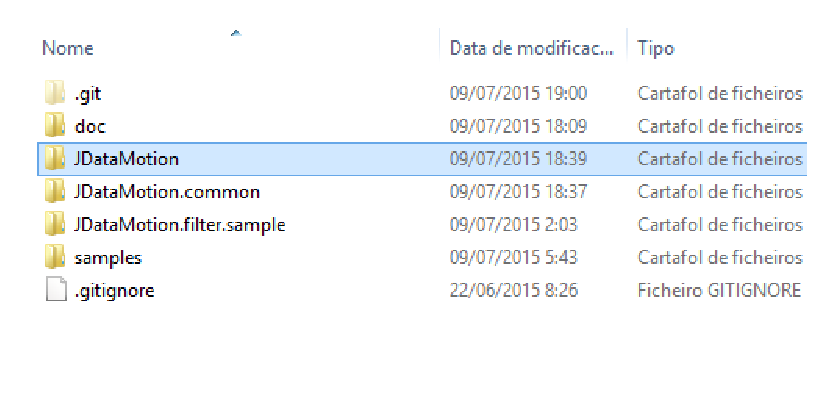
\includegraphics[width=\textwidth,height=\textheight,keepaspectratio]{figuras/carpetaAplicacion}
\caption{Carpeta da aplicación JDataMotinon (seleccionada)}
\label{carpetaAplicacion}
\end{figure}

Unha vez que escollemos o emprazamento para a aplicación, accedemos a ela e seguimos estes pasos en función do noso sistema operativo:

\begin{itemize}
\item Para sistemas baseados en Windows, buscamos o ficheiro ``run.bat''. Podemos crear un acceso directo a este arquivo en calquera outro lugar, pero non copialo ou movelo a outro directorio.
\item Para sistemas baseados en Linux, abrimos primeiramente un terminal e desprazámonos ata o directorio da aplicación. Introducimos o comando ``sudo chmod +x run.sh'' e introducimos o contrasinal de administrador. Podemos crear un lanzador cara este arquivo en calquera outro lugar, pero non copialo ou movelo a outro directorio. Executamos o arquivo con ./run.sh
\end{itemize}

En calquera dos dous casos, apareceranos unha ventá parecida á da figura \ref{inicial}.

\begin{figure}
\centering
\includegraphics[width=\textwidth,height=\textheight,keepaspectratio]{figuras/inicial}
\caption{Ventá de JDataMotion}
\label{inicial}
\end{figure}

\section{Utilización}

Para comezar a traballar temos dúas vías. A primeira é crear un novo experimento importando un ficheiro en formato .csv ou .arff. Para isto iríamos a Ficheiro \textgreater{} Importar ficheiro. A continuación buscaríamos no explorador un ficheiro cunha extensión válida (ver figura \ref{importarFicheiro}).

\begin{figure}
\centering
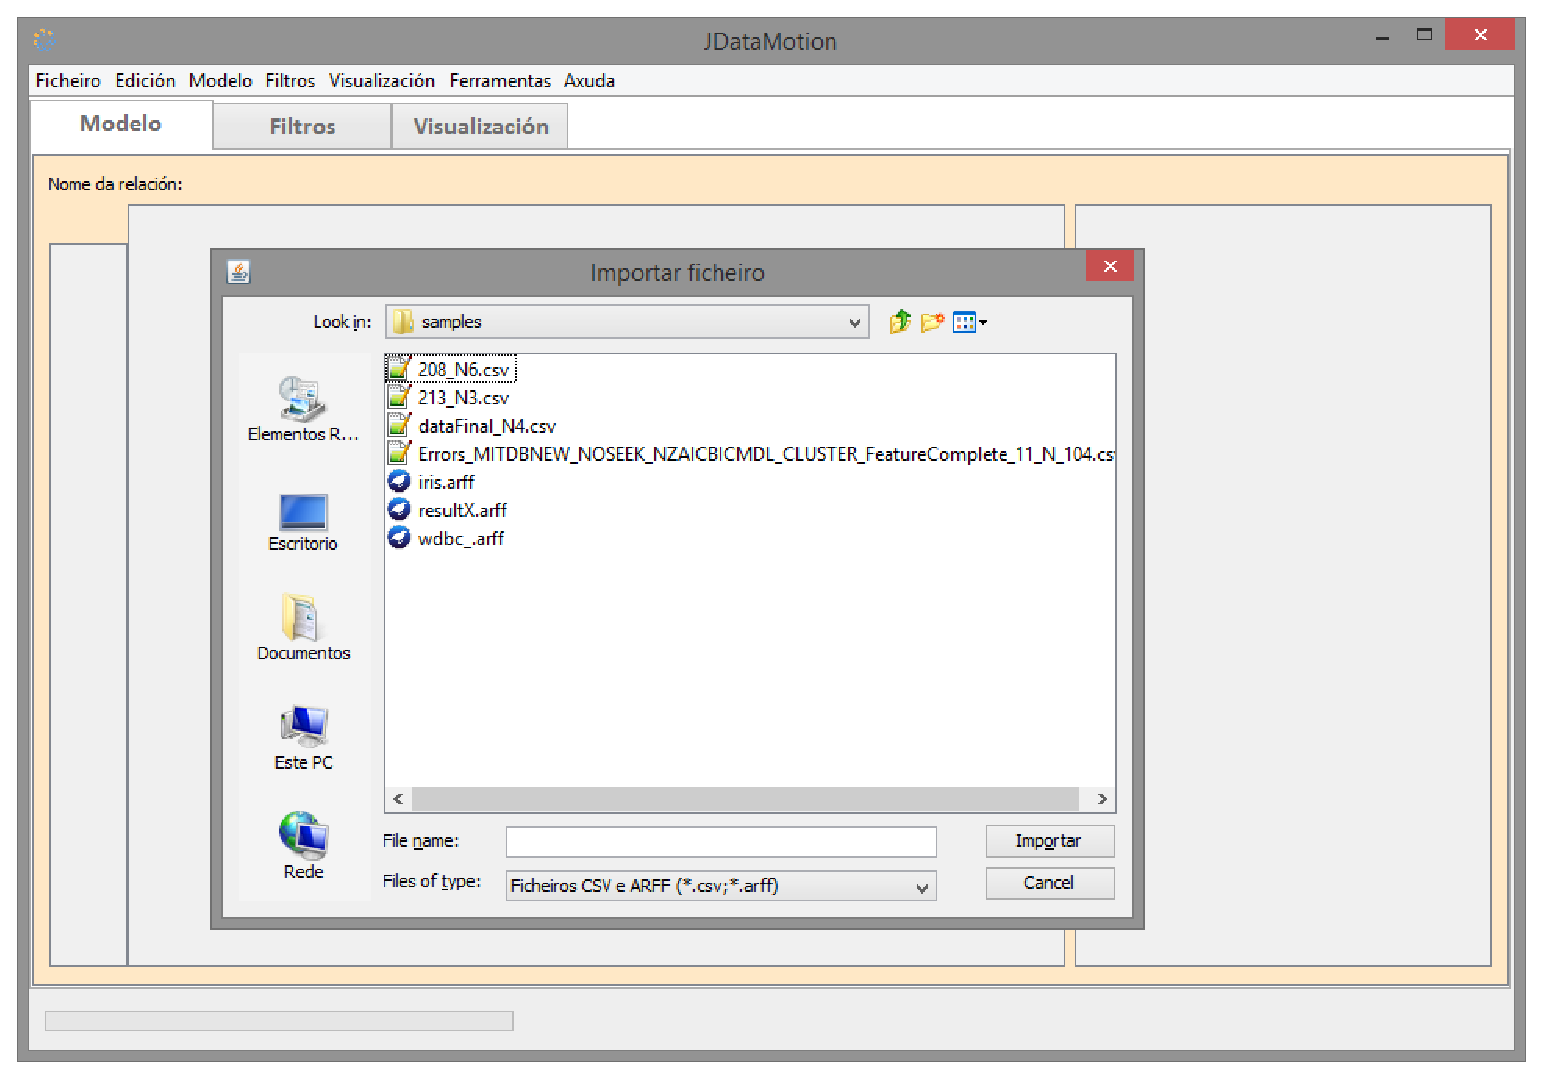
\includegraphics[width=\textwidth,height=\textheight,keepaspectratio]{figuras/importarFicheiro}
\caption{Importación dun ficheiro}
\label{importarFicheiro}
\end{figure}

A outra forma de comezar a traballar é abrir unha sesión gardada previamente. Para isto iríamos a Ficheiro \textgreater{} Abrir sesión. A continuación buscaríamos no explorador un ficheiro coa extensión .jdms (ver figura \ref{abrirSesion}).

\begin{figure}
\centering
\includegraphics[width=\textwidth,height=\textheight,keepaspectratio]{figuras/abrirSesion}
\caption{Abrir unha sesión}
\label{abrirSesion}
\end{figure}

\subsection{Modelo}

O menú Modelo encherase representando os atributos nas cabeceiras da táboa, e os datos como filas da mesma (ver figura \ref{manualModelo}).

\begin{figure}
\centering
\includegraphics[width=\textwidth,height=\textheight,keepaspectratio]{figuras/manualModelo}
\caption{Modelo con datos}
\label{manualModelo}
\end{figure}

Se pinchamos nalgunha das cabeceiras da táboa veremos no panel da dereita un resumo dos datos que contén, ademais dun histograma cos valores que toma. Podemos facer que este histograma agrupe as barras segundo un atributo nominal (tamén chamado atributo de clase). Para isto deberemos especificar cal queremos usar, dirixíndonos ao menú Visualización \textgreater{} Establecer atributo nominal representado, e seleccionando o atributo que prefiramos. Se non aparece o que se desexa usar, teremos que cambiarlle o tipo a ``nominal'' para que estea dispoñible. O resultado será algo parecido ao da figura \ref{histogramaNominal}.

\begin{figure}
\centering
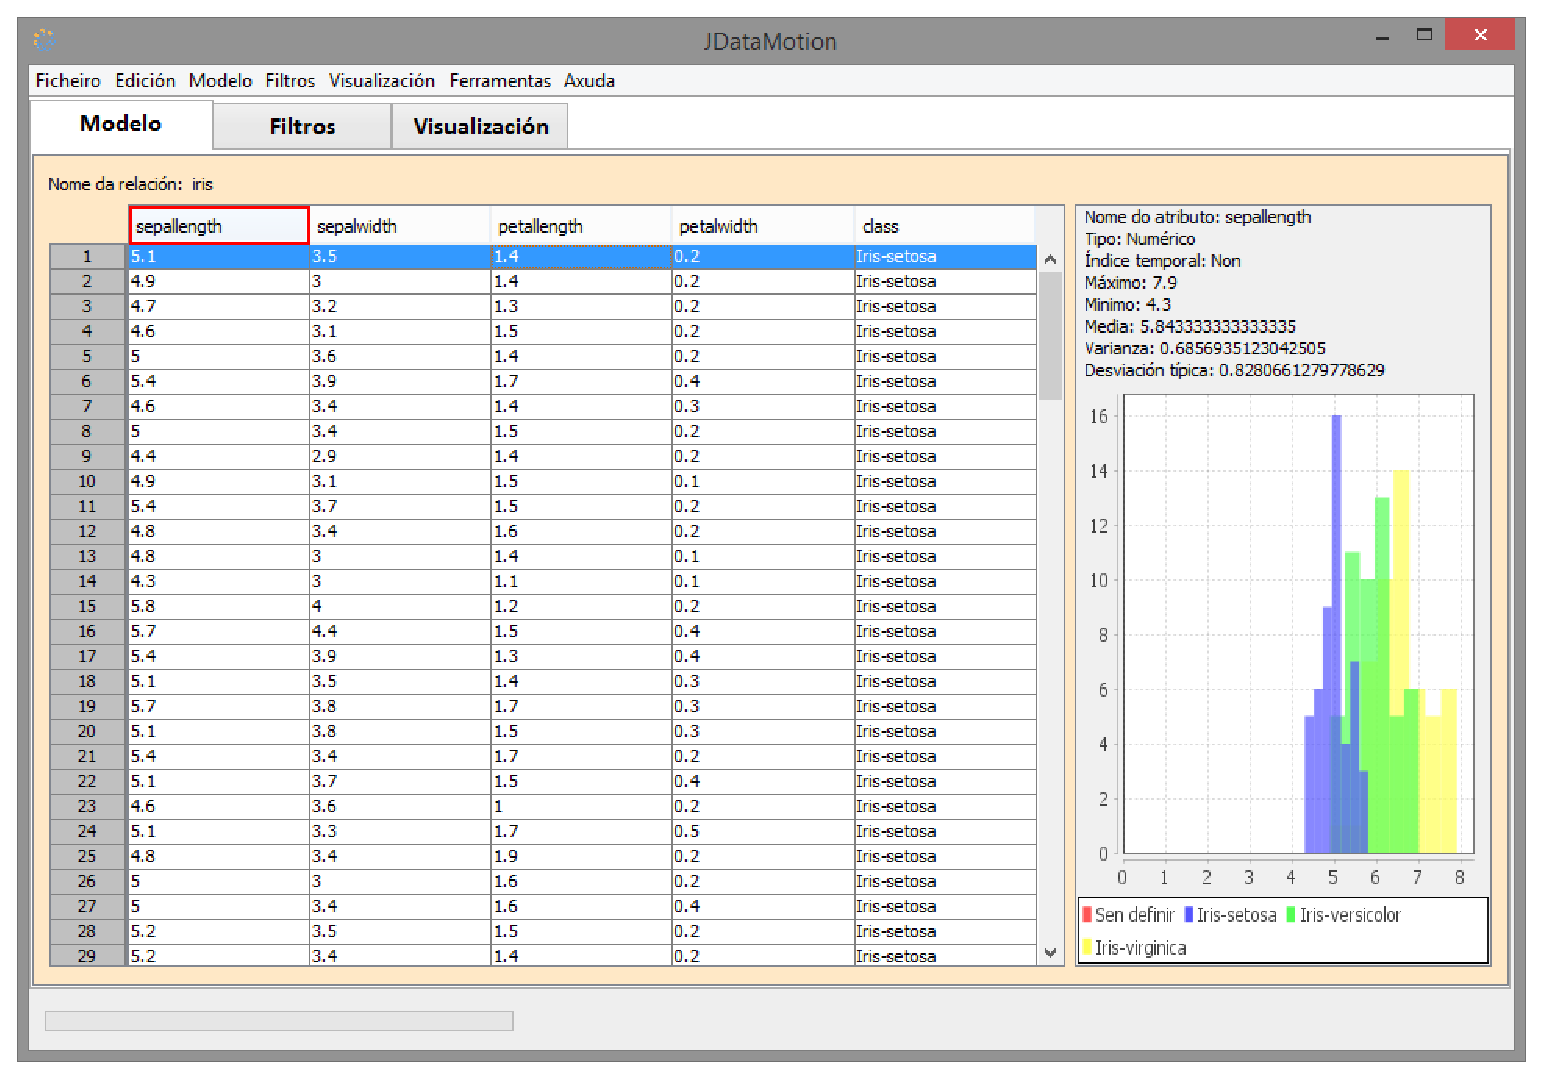
\includegraphics[width=\textwidth,height=\textheight,keepaspectratio]{figuras/histogramaNominal}
\caption{Histograma que usa un atributo nominal}
\label{histogramaNominal}
\end{figure}

Para mudar o tipo dun atributo debemos premer na súa cabeceira co botón secundario. Sairá un menú emerxente con varios ítems (ver figura \ref{menuAtributo}), iremos a Tipo e a continuación seleccionaremos o tipo ao que queremos que se converta o atributo e máis os seus datos. A conversión deixará campos baleiros onde non sexa capaz de realizar a conversión (por exemplo, se pasamos a numérico un atributo que ten un texto nunha celda).

\begin{figure}
\centering
\includegraphics[width=\textwidth,height=\textheight,keepaspectratio]{figuras/menuAtributo}
\caption{Menú emerxente dos atributos}
\label{menuAtributo}
\end{figure}

No menú emerxente dos atributos tamén temos a opción Agochar columna, que a quitará do menú sen eliminar os seus elementos. Para restablecer as columnas ocultadas, iremos a Modelo \textgreater{} Amosar todas as columnas. A última posibilidade deste menú contextual permítenos asignar o índice temporal ao atributo no que se premeu. O atributo debe ser de tipo numérico, ou de tipo String contendo valores nun formato de tempo ([[HH:]mm:]ss). Establecendo o índice temporal poderemos facer que as reproducións posteriores sigan a orde do atributo que é o índice temporal.

Pulsando dúas veces unha cela da táboa podemos editar o seu valor. Se o atributo é de tipo nominal, despregarásenos unha lista dos posibles valores que pode tomar. Se o novo dato que inserimos nesa cela non é compatible co atributo ao que pertence notificarásenos o erro.

Podemos engadir ou eliminar tanto filas (instancias) coma columnas (atributos) á táboa do Modelo.

Para engadir filas iremos a Modelo \textgreater{} Engadir instancia. A nova instancia figura baleira ao final da táboa (ver figura \ref{engadirInstancia}). Podémoslle asignar valores premendo dúas veces nas celas que a compoñen.

\begin{figure}
\centering
\includegraphics[width=\textwidth,height=\textheight,keepaspectratio]{figuras/engadirInstancia}
\caption{Resultado de engadir instancia}
\label{engadirInstancia}
\end{figure}

Se desexamos eliminar un conxunto de filas, primeiro teremos que seleccionalas na táboa. Pódense seleccionar varias mantendo pulsada a tecla Control, ou pulsar a tecla Mayus e seleccionar dúas filas, de xeito que tamén queden seleccionadas as filas que as separan. Unha vez teñamos a selección feita, iremos a Modelo \textgreater{} Eliminar instancias, para descartalas.

Os atributos engádense por medio de Modelo \textgreater{} Engadir atributo. Ao facelo, a táboa contará cun atributo máis ao final, chamado ``novoAtributo''. Este atributo novo é por defecto de tipo String. Esto podémolo apreciar na figura \ref{engadirAtributo}.

\begin{figure}
\centering
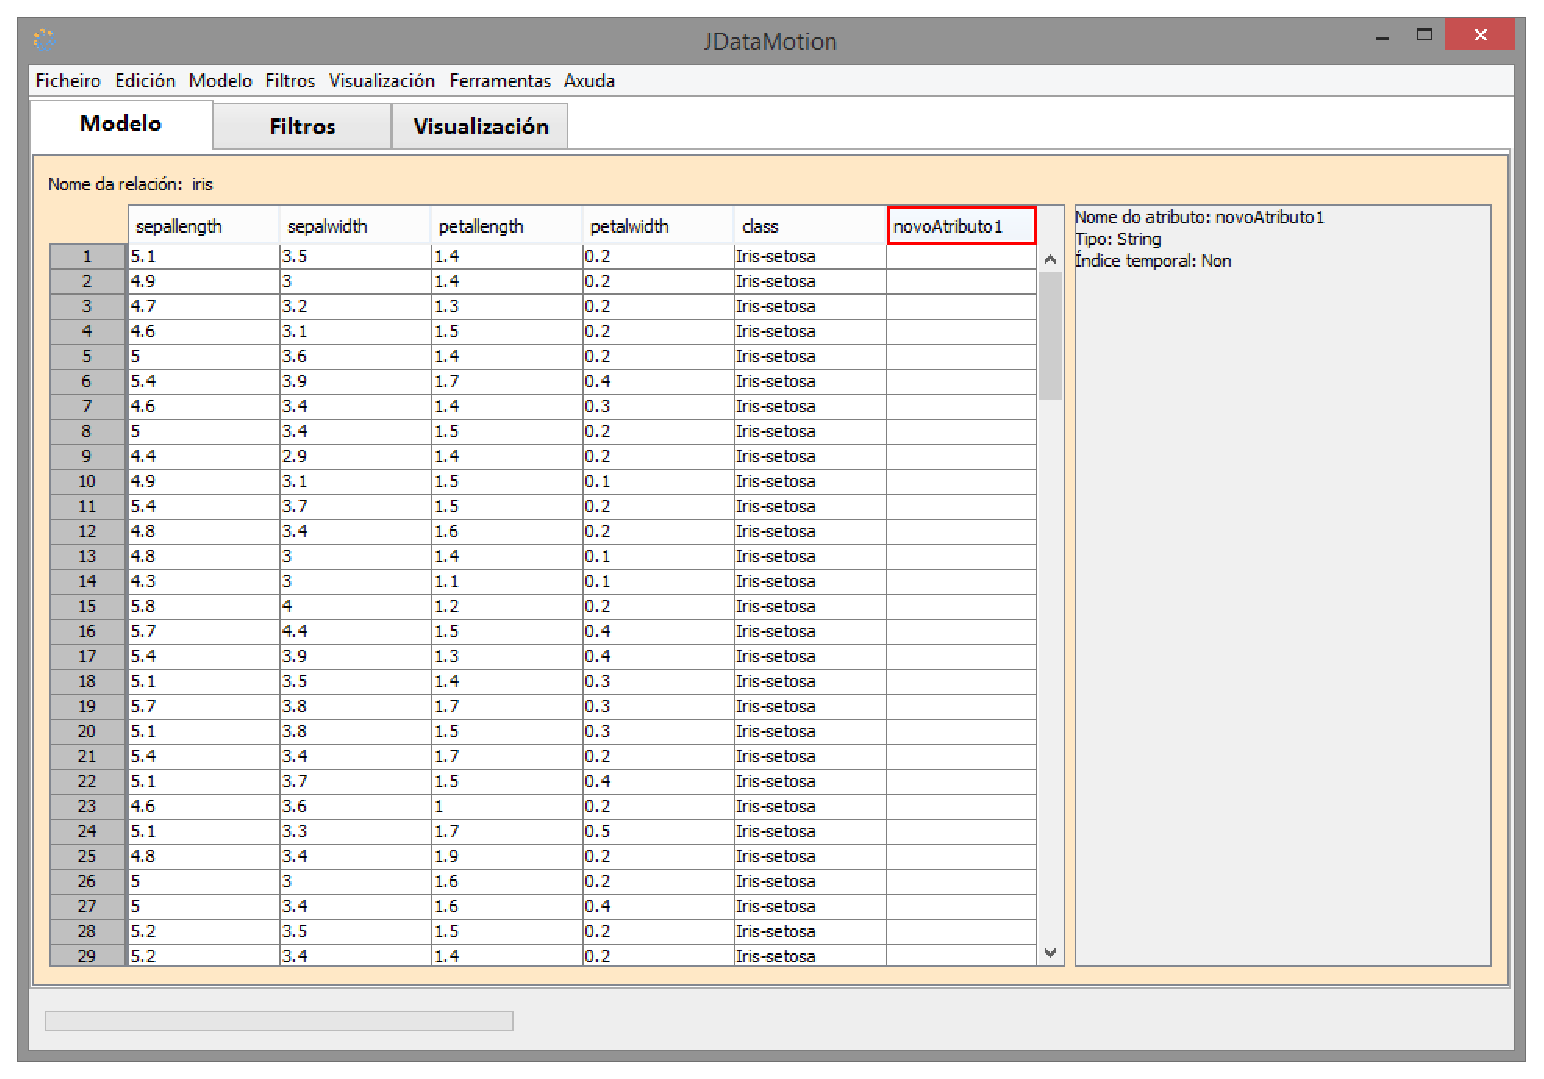
\includegraphics[width=\textwidth,height=\textheight,keepaspectratio]{figuras/engadirAtributo}
\caption{Resultado de engadir atributo}
\label{engadirAtributo}
\end{figure}

Podemos eliminar atributos seleccionándoos e, a continuación, indo a Modelo \textgreater{} Eliminar atributo.

Tamén podemos mudar o nome dun atributo seleccionándoo e indo a Modelo \textgreater{} Renomear atributo. Inserimos o novo nome do atributo e aceptamos. Non se deben duplicar nomes de atributos, se o novo nome do atributo xa existe, o sistema avisaranos do erro.

Por último, podemos cambiarlle o nome á relación de datos coa que estamos traballando con Modelo \textgreater{} Mudar nome da relación.

Para descartar todos os cambios e recargar o ficheiro orixinal podemos usar a función Modelo \textgreater{} Restaurar.

\subsection{Filtros}

Unha vez lle demos formato ou completemos os datos do Modelo, podemos avanzar cara a segunda lapela da aplicación, que amosará o menú de Filtros, tal e como se amosa na figura \ref{manualFiltros}

\begin{figure}
\centering
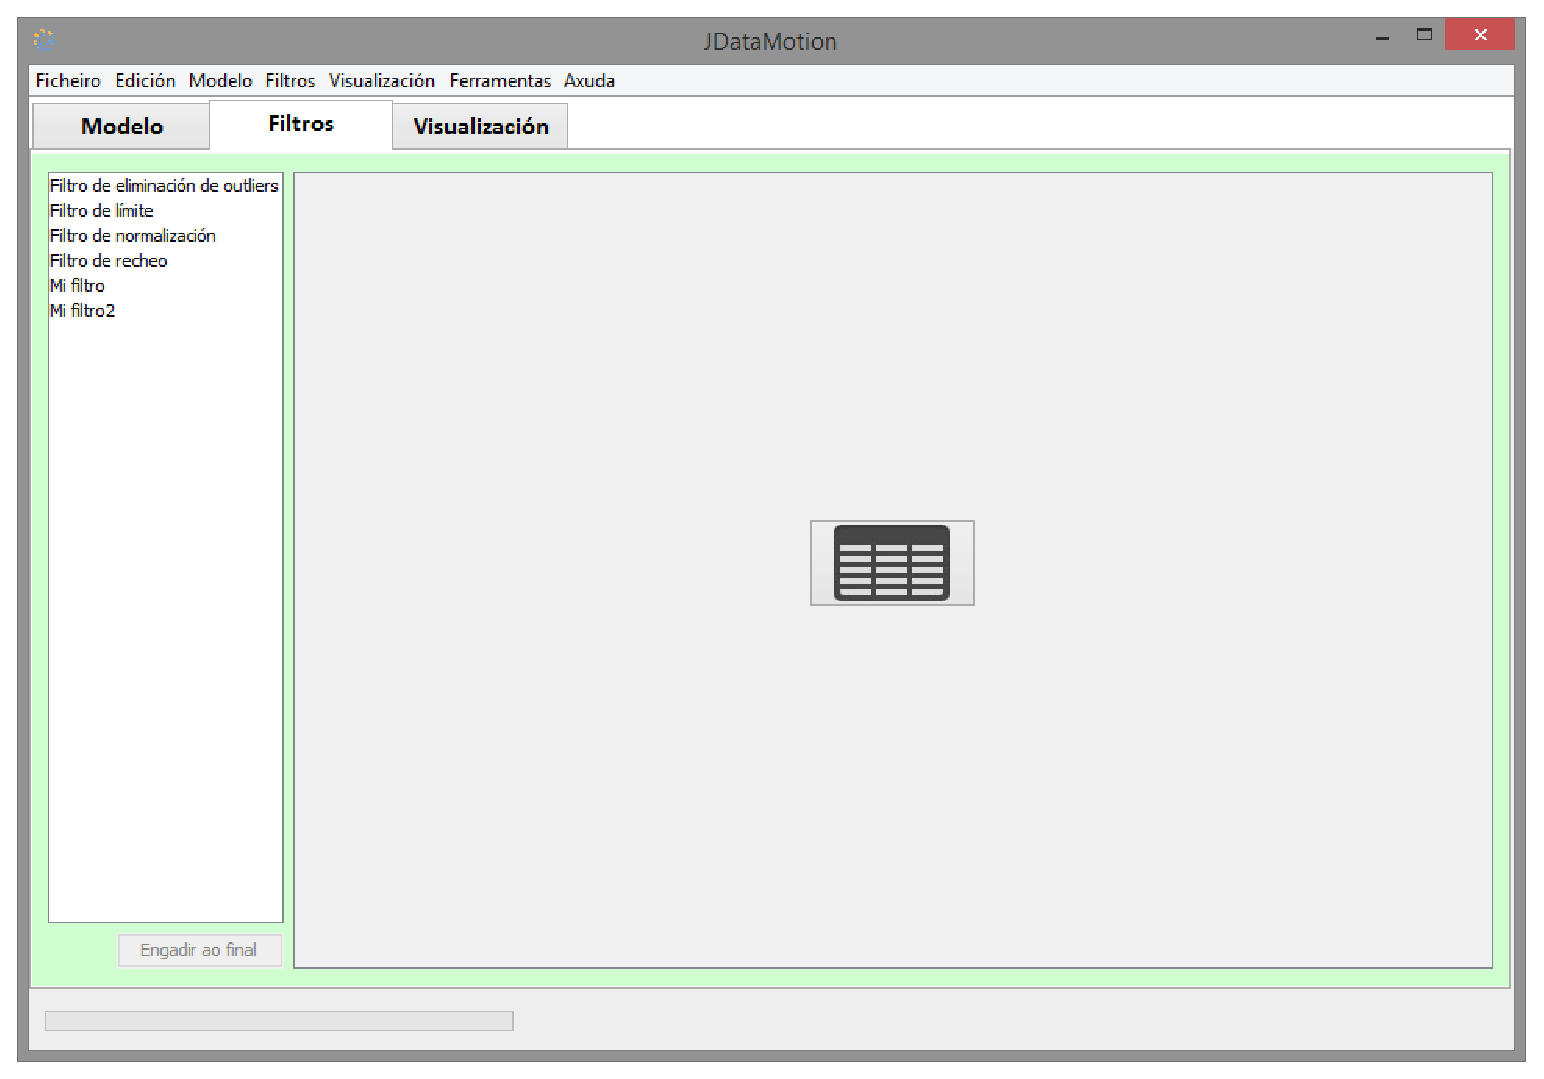
\includegraphics[width=\textwidth,height=\textheight,keepaspectratio]{figuras/manualFiltros}
\caption{Menú Filtros}
\label{manualFiltros}
\end{figure}

Neste menú poderemos seleccionar filtros da lista situada á esquerda, e premer en ``Engadir ao final'' para situar o filtro na secuencia. A medida que engadamos filtros esta secuencia irá aumentando (ver figura \ref{secuenciaFiltros}).

\begin{figure}
\centering
\includegraphics[width=\textwidth,height=\textheight,keepaspectratio]{figuras/secuenciaFiltros}
\caption{Secuencia de filtros}
\label{secuenciaFiltros}
\end{figure}

Dentro do panel que ilustra a secuencia temos varios ítems. Por unha parte, a primeira icona empezando pola esquerda pódese premer, para ampliar nunha ventá aparte o modelo de datos do que se parte antes de aplicar ningún filtro.

Os embudes verdes representan os filtros engadidos. Se saen cun signo de admiración en amarelo, significa que algún parámetro do filtro está sen definir, e polo tanto o filtro non se está aplicando realmente.

Para configurar un filtro temos que premer a primeira das iconas que ten baixo a súa representación (uns engrenaxes negros). Aparecerá unha ventá para inserir os valores que necesita o filtro. Unha vez os insertemos todos, o icono de ``filtro sen configurar'' desaparecerá (ver figura \ref{filtrosConfigurados}).

\begin{figure}
\centering
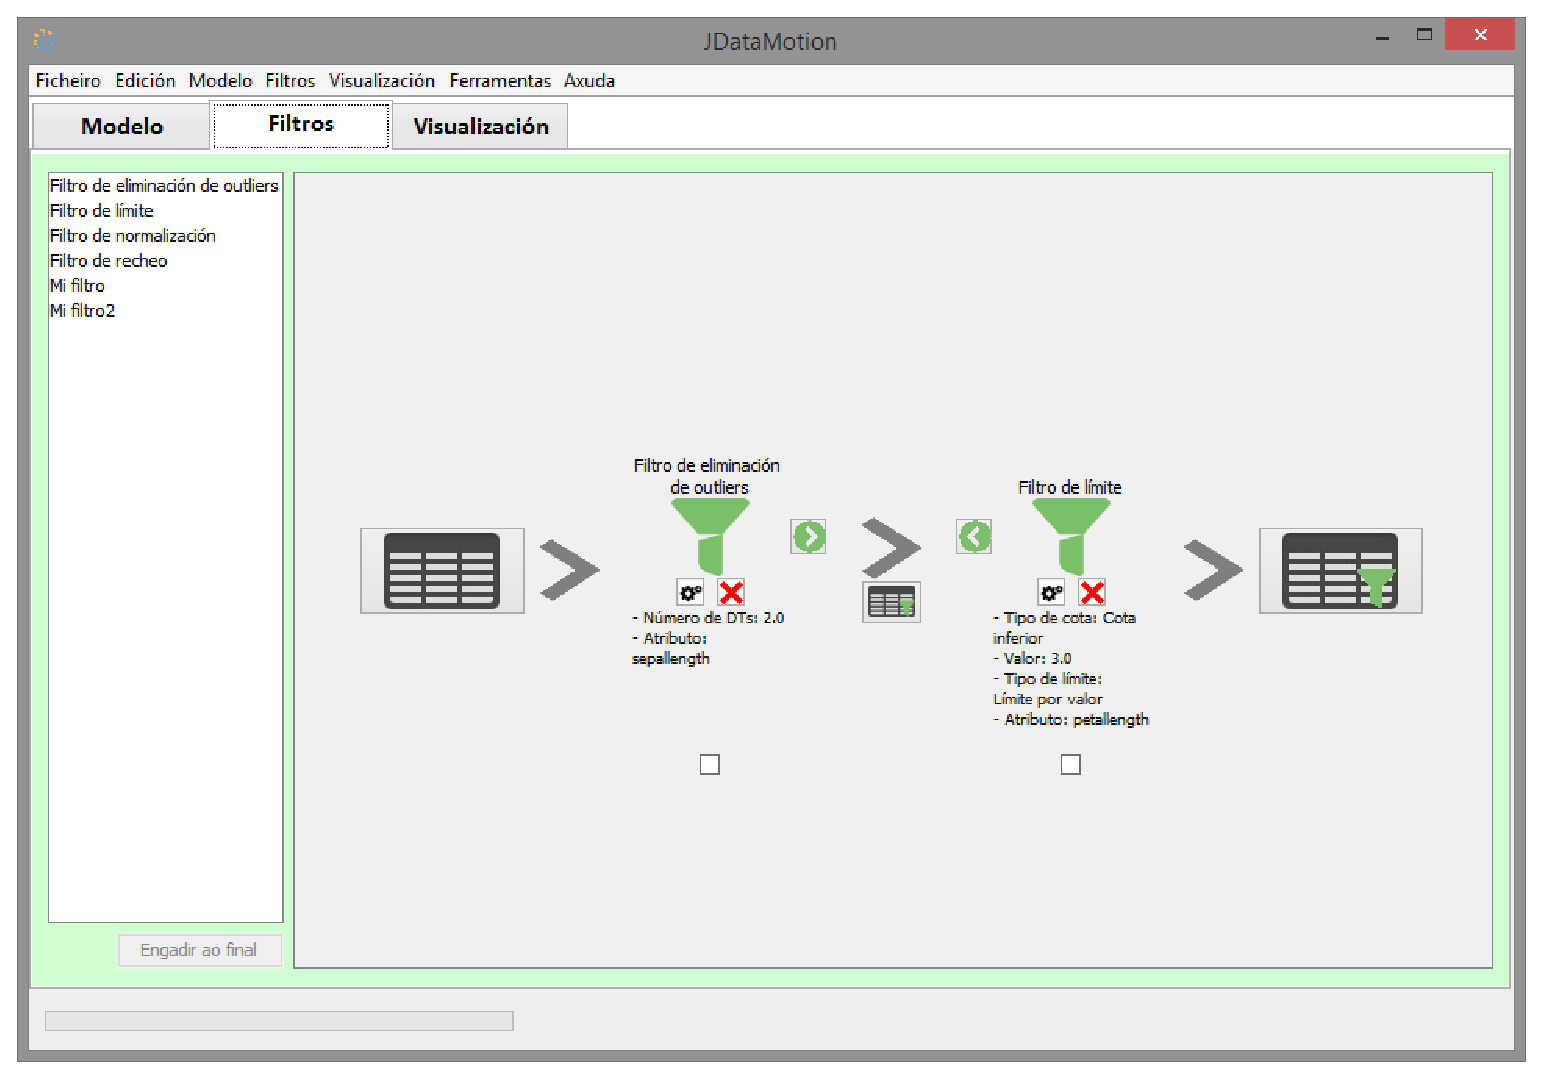
\includegraphics[width=\textwidth,height=\textheight,keepaspectratio]{figuras/filtrosConfigurados}
\caption{Filtros configurados}
\label{filtrosConfigurados}
\end{figure}

A icona contigua á de configuración (cunhas aspas vermellas) serve para eliminar o filtro da secuencia, anulando os seus efectos.

A frecha verde que cada filtro pode ter aos seus lados permite mover o filtro na secuencia, alterando a orde de aplicación.

Entre cada dous filtros consecutivos temos unha icona de táboa de menor tamaño. Premer nela amósanos como se atopa o modelo ata ese punto, tras aplicarse todos os filtros á esquerda pero ningún da dereita aínda. Trátase da representación dun modelo parcial.

Por último, a icona á dereita da secuencia (unha táboa cun embude) mostra o modelo final, tras a aplicación de toda a secuencia de filtros. Este modelo final será co que se vaia a traballar no último menú da aplicación.

Podemos seleccionar filtros utilizando o checkbox ou cadro seleccionable que teñen debaixo. Seleccionar filtros permitiranos utilizar a opción Filtros \textgreater{} Exportar filtros seleccionados. Ao facelo, pedirase un directorio e un nome de arquivo no que se almacenarán os filtros marcados baixo un arquivo de extensión .jdmf.

Eses filtros poden ser logo recuperados en calquera sesión. Se os volvemos a importar, engadiranse ao final da secuencia, tal e como podemos observar na figura \ref{filtrosRecuperados}.

\begin{figure}
\centering
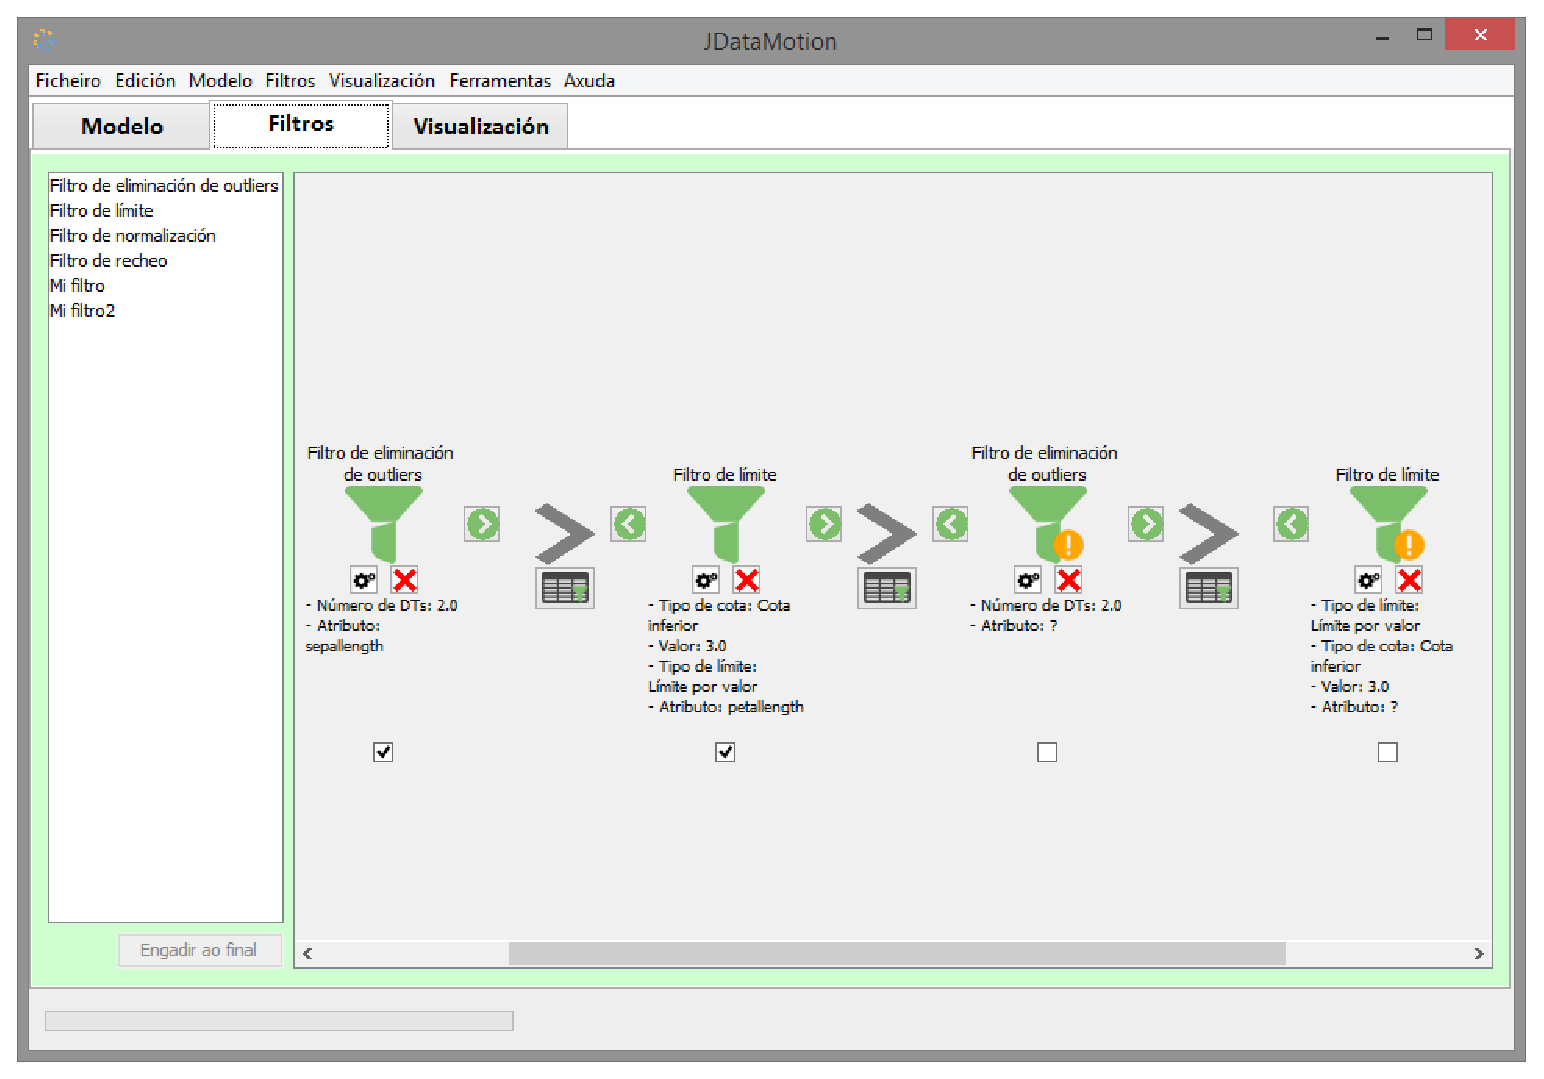
\includegraphics[width=\textwidth,height=\textheight,keepaspectratio]{figuras/filtrosRecuperados}
\caption{Filtros exportados e importados}
\label{filtrosRecuperados}
\end{figure}

Nótese que para preservar a integridade dos filtros entre experimentos distintos, estes perden o atributo sobre o que actúan ao seren importados, co cal temos que volver a configurar este parámetro.

Por último, podemos aumentar a lista de filtros dispoñibles na lista da esquerda importándoos dende unha libraría en formato .jar. Para isto, iremos a Filtros \textgreater{} Importar filtro dende JAR e indicaremos no explorador que ficheiro queremos analizar na procura de filtros. Nótese que un filtro é calquera clase que implemente a interface IFilter que proporciona este proxecto.

\subsection{Visualización}

Chegados a este punto xa temos os datos do ficheiro preprocesados e filtrados, así que agora imos a representalos dinamicamente. Para iso accedemos á última lapela da aplicación, que nos amosará o Menú Visualización, que será parecido ao da figura \ref{manualVisualizacion}.

\begin{figure}
\centering
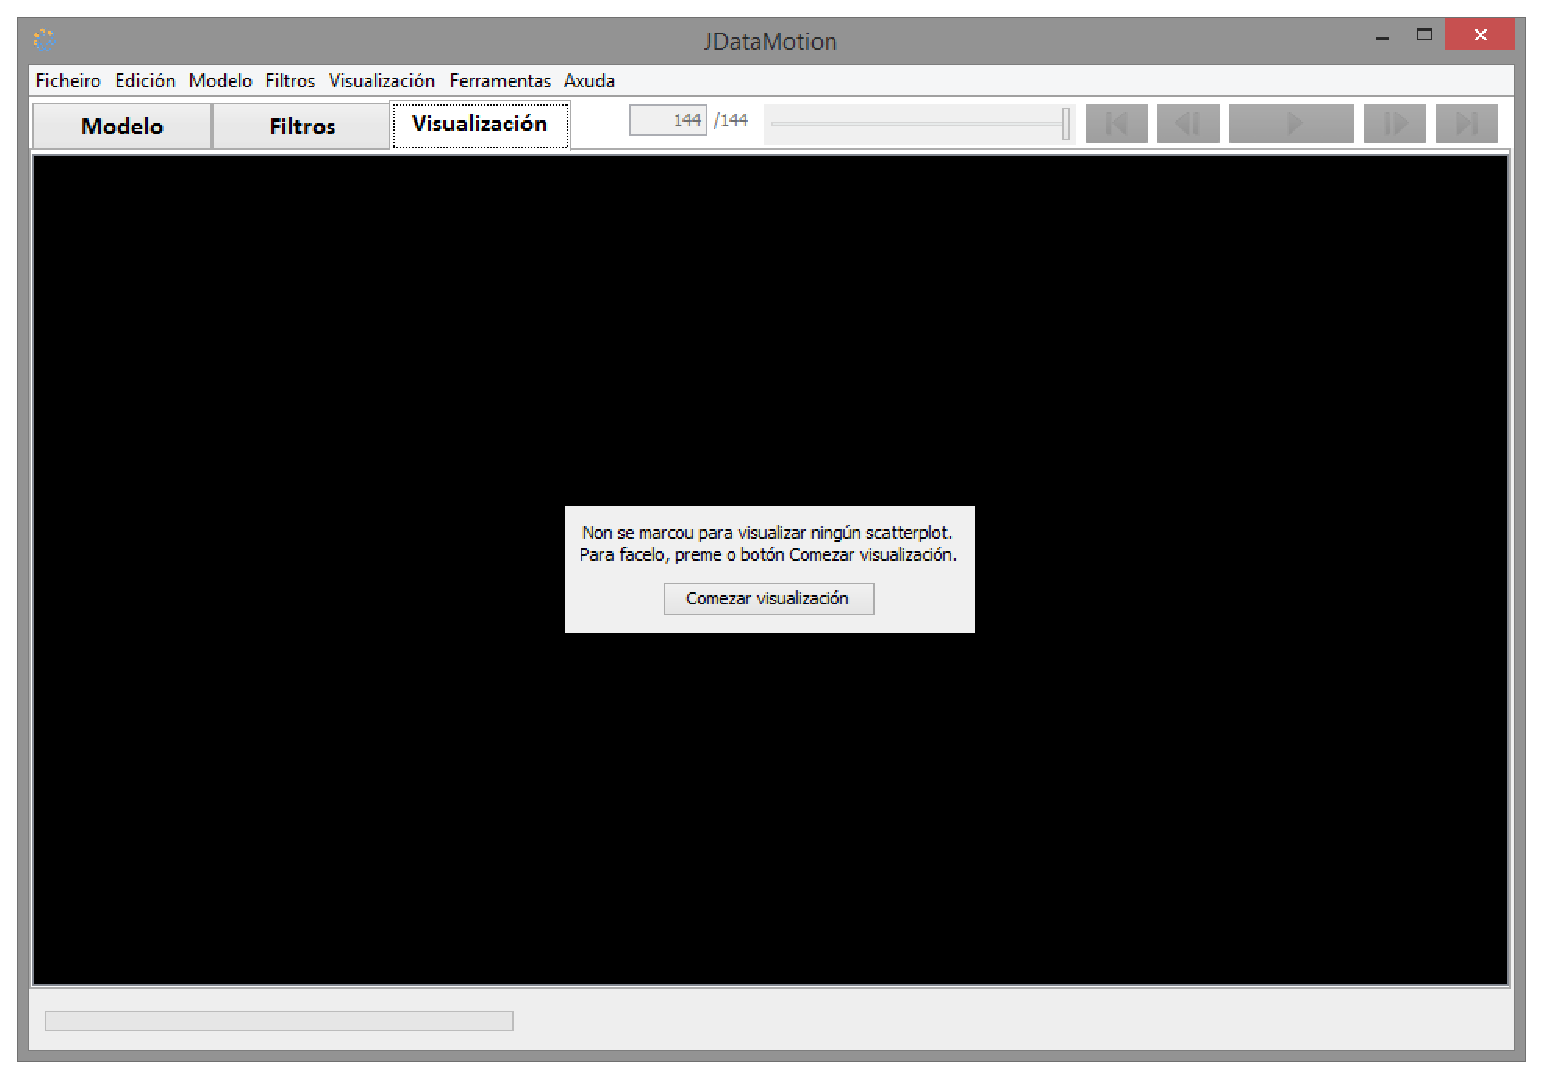
\includegraphics[width=\textwidth,height=\textheight,keepaspectratio]{figuras/manualVisualizacion}
\caption{Menú Visualización}
\label{manualVisualizacion}
\end{figure}

A primeira vez que accedemos a este menú non haberá nada, e suxerirannos engadir algún scatterplot ou diagrama de dispersión por medio do botón ``Comezar visualización''. Premémolo e veremos unha matriz parecida á da figura \ref{matrizVisualizacion}.

\begin{figure}
\centering
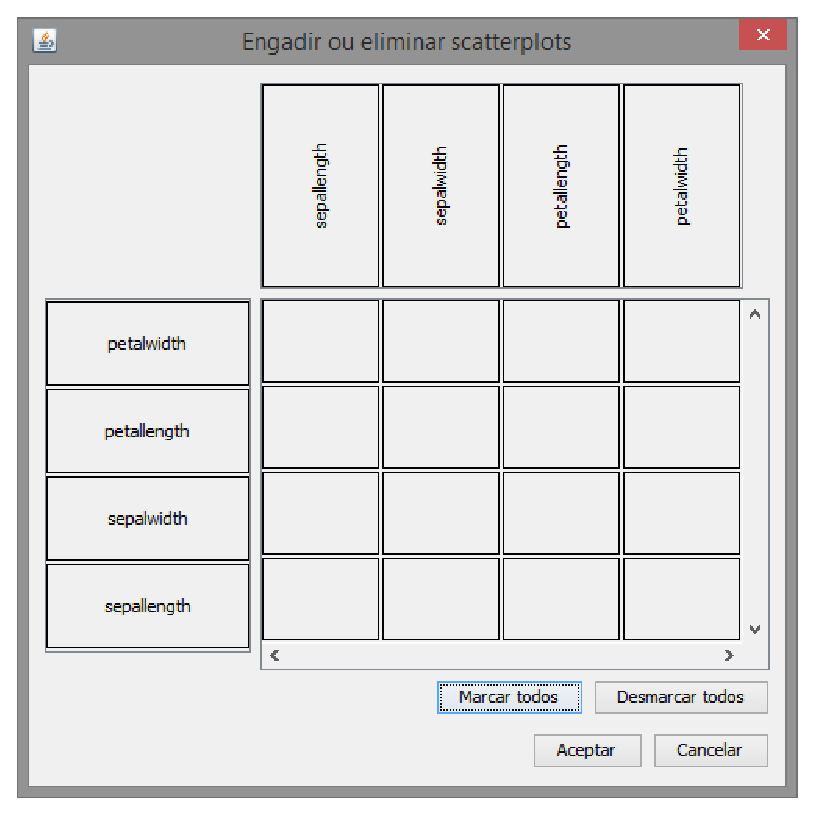
\includegraphics[width=\textwidth,height=\textheight,keepaspectratio]{figuras/matrizVisualizacion}
\caption{Matriz seleccionable de diagramas}
\label{matrizVisualizacion}
\end{figure}

Esta matriz amosa tantas celas como posibles diagramas se poden visualizar. Cada diagrama é a combinación de dous atributos numéricos, un para definir os valores das abscisas (o atributo da columna) e outro para definir os valores das ordenadas (o atributo da fila). Podemos seleccionar e deseleccionar diagramas nesta ventá individualmente (iranse marcando en amarelo as que se desexen visualizar) ou seleccionalas/deseleccionalas todas á vez.

Unha vez fagamos a nosa selección, o menú de Visualización debería encherse con algo semellante ao da figura \ref{matrizChea}.

\begin{figure}
\centering
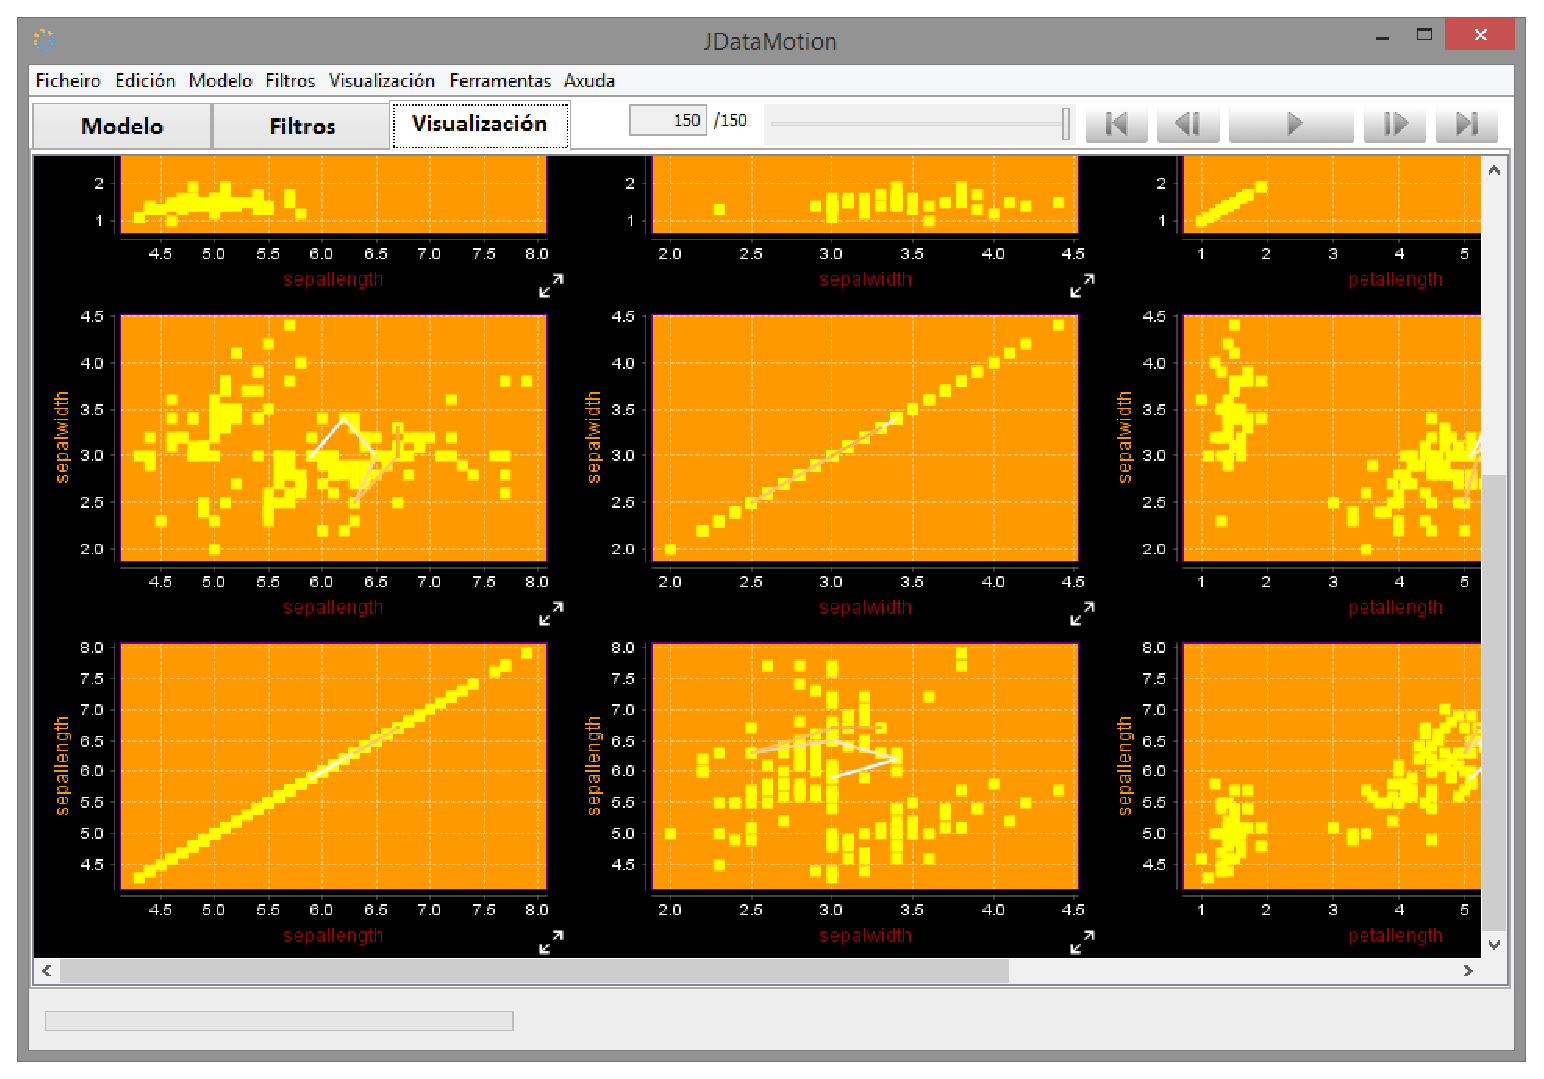
\includegraphics[width=\textwidth,height=\textheight,keepaspectratio]{figuras/matrizChea}
\caption{Matriz de visualización}
\label{matrizChea}
\end{figure}

Todos os diagramas que agora están no Menú de Visualización teñen unha icona con forma de dúas frechas na esquina sueste. Podemos premelos para ampliar un ou varios diagramas nunha ventá aparte.

Se seleccionamos un atributo nominal durante o noso paso polo menú Modelo, ou mesmo se o seleccionamos agora, os diagramas amosarán os puntos agrupados segundo un atributo que será tomado como atributo de clase, tal e como se mostra na figura \ref{diagramasNominais}.

\begin{figure}
\centering
\includegraphics[width=\textwidth,height=\textheight,keepaspectratio]{figuras/diagramasNominais}
\caption{Diagramas con atributo de clase}
\label{diagramasNominais}
\end{figure}

Para volver á ventá para seleccionar que diagramas queremos ver, podemos acceder por medio de Visualización \textgreater{} Engadir ou eliminar scatterplots.

Cada diagrama de dispersión realiza as seguintes funcionalidades:

\begin{description}
\item[Botón secundario no diagrama \textgreater{} Copiar:] \hfill
Garda unha captura do diagrama no portapapeis.
\item[Botón secundario no diagrama \textgreater{} Gardar como \textgreater{}PNG:] \hfill
Garda unha captura do diagrama nun ficheiro de imaxe PNG.
\item[Botón secundario no diagrama \textgreater{} Imprimir:] \hfill
Imprime a captura do diagrama.
\item[Botón secundario no diagrama \textgreater{} Acercar:] \hfill
Aumenta a escala da ventá de visualización do diagrama en termos dun dos eixos ou dos dous.
\item[Botón secundario no diagrama \textgreater{} Alonxar:] \hfill
Diminúe a escala da ventá de visualización do diagrama en termos dun dos eixos ou dos dous.
\item[Botón secundario no diagrama \textgreater{} Escala automática:] \hfill
Reaxusta a escala da ventá de visualización para que abarque de forma exacta a totalidade dos puntos. Pode tamén aplicarse só sobre un dos eixos ou sobre os dous.

\item[Botón Control + arrastrar o diagrama:] \hfill
Reposiciona a ventá que enfoca o diagrama, seguindo a dirección do cursor.
\item[Arrastre dentro do diagrama:] \hfill
Escala a ventá que enfoca o diagrama, de tal forma que se centre no cadrado debuxado durante o arrastre.
\item[Xirar a roda do rato co cursor encima dun diagrama:] \hfill
Escala a ventá de visualización dese diagrama.
\item[Premer nun punto do diagrama:] \hfill
Abre un cadro emerxente que describe todos os atributos da instancia representada nese punto. Ademais, se nesa posición hai varios puntos superpostos, resalta cunha circunferencia eses puntos nos demais diagramas. Os puntos rodeados por circunferencias da mesma cor representarán á mesma instancia en proxeccións diferentes. Podemos apreciar este proceso na figura \ref{resaltarPuntoSeleccionado}.
\begin{figure}
\centering
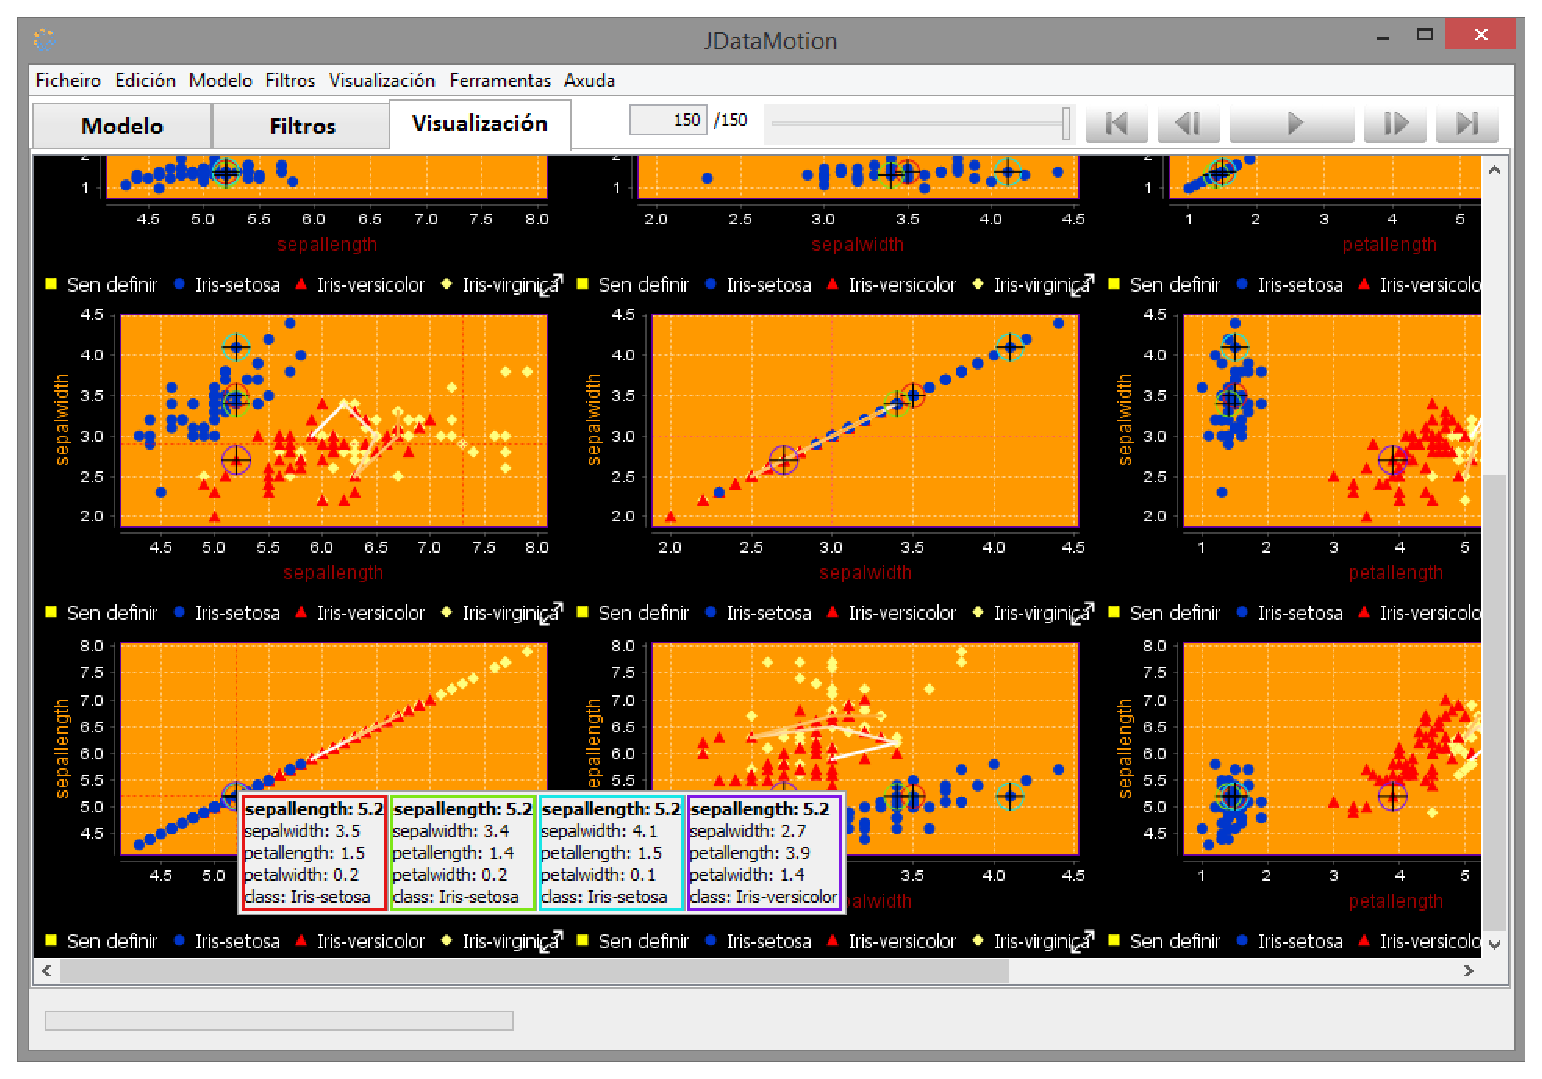
\includegraphics[width=\textwidth,height=\textheight,keepaspectratio]{figuras/resaltarPuntoSeleccionado}
\caption{Selecciín dun punto nun diagrama}
\label{resaltarPuntoSeleccionado}
\end{figure}

\item[Botón secundario no diagrama \textgreater{} Propiedades:] \hfill
Abre unha ventá, similar á da figura \ref{propiedadesDiagramas}, que nos permitirá engadir as nosas preferencias gráficas con respecto a esta sección. Nela poderemos configurar os seguintes aspectos:
\begin{itemize}
\item Fonte dos títulos dos diagramas (só diagramas ampliados)
\item Cor dos títulos dos diagramas (só diagramas ampliados)
\item Fonte do eixo horizontal, que é a fonte coa que se representa o atributo das abscisas.
\item Fonte do eixo vertical, que é a fonte coa que se representa o atributo das ordenadas.
\item Cor do eixo horizontal, que é a cor coa que se representa o atributo das abscisas.
\item Cor do eixo vertical, que é a cor coa que se representa o atributo das ordenadas.
\item Visualizar etiquetas de graduación de escala no eixo horizontal, que activa ou desactiva as etiquetas numéricas das abscisas.
\item Visualizar marcas de graduación de escala no eixo horizontal, que activa ou desactiva as marcas das abscisas para sinalar intervalos.
\item Visualizar etiquetas de graduación de escala no eixo vertical, que activa ou desactiva as etiquetas numéricas das ordenadas.
\item Visualizar marcas de graduación de escala no eixo vertical, que activa ou desactiva as marcas das ordenadas para sinalar intervalos.
\item Fonte das etiquetas de graduación de escala no eixo horizontal, que son as etiquetas numéricas das abscisas.
\item Fonte das etiquetas de graduación de escala no eixo vertical, que son as etiquetas numéricas das ordenadas.
\item Estilo do trazo do bordo, que é o grosor da liña que bordea o diagrama
\item Cor do bordo, que é a cor da liña que bordea o diagrama.
\item Cor de fondo (lapela Trazo), que é a cor do lenzo sobre o que se visualizan os puntos dentro do diagrama.
\item Anti-aliasing, para activar ou desactivar o anti-aliasing ao representar os puntos.
\item Cor de fondo (lapela Outro), que é a cor do fondo do Menú de Visualización
\item Cor das series, que é a cor que se utilizará para pintar cada grupo asociado a un atributo de clases.
\item Estilo do trazo das series, que é a forma (estrela ou polígono de n vértices) que se utilizará para pintar cada grupo asociado a un atributo de clases.
\end{itemize}
\begin{figure}
\centering
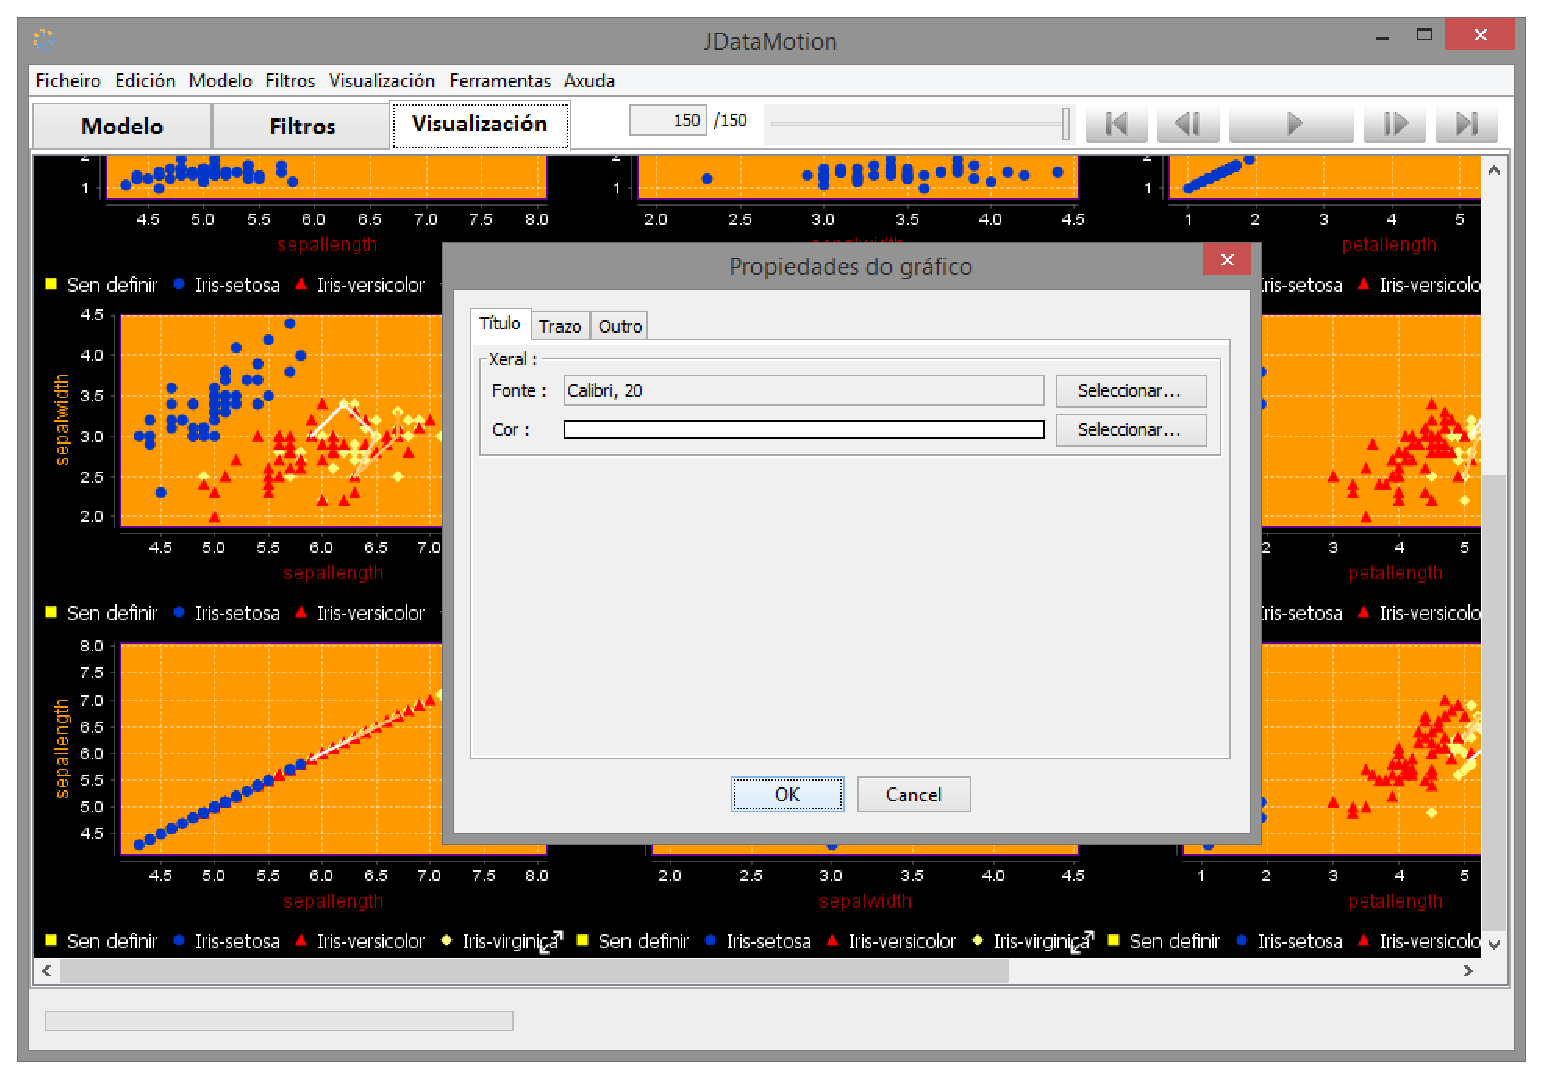
\includegraphics[width=\textwidth,height=\textheight,keepaspectratio]{figuras/propiedadesDiagramas}
\caption{Configuración das preferencias gráficas}
\label{propiedadesDiagramas}
\end{figure}
\end{description}

Para configurar o tipo de reprodución que queremos, iremos a Visualización \textgreater{} Configurar reprodutor. Obteremos un menú similar ao da figura \ref{configurarReproducion}.

\begin{figure}
\centering
\includegraphics[width=\textwidth,height=\textheight,keepaspectratio]{figuras/configurarReproducion}
\caption{Menú de configuración do reprodutor}
\label{configurarReproducion}
\end{figure}

Neste menú hai varios aspectos interesantes. Por unha parte, a orde de reprodución definirá a orde na que as instancias serán visualizadas. Por defecto ten o valor ``Orde do modelo'', que as representa a intervalos de tempo iguais en función do seu índice de fila. Sen embargo, se seleccionamos temos marcado un atributo como índice temporal, poderemos seleccionar neste menú as opcións ``Orde dos índices temporais numéricos'', que representaría as instancias en intervalos iguais de tempo pero ordenándoas segundo o atributo temporal, ou ``Orde dos índices temporais numéricos ponderados'', que ademais de ordenar as instancias polo atributo temporal, lles asigna unha marca temporal proporcional ao valor deste. É dicir, que o índice temporal tería un peso con respecto aos demáis. Se o índice temporal é un String representando un número de segundos, minutos ou horas, recoméndase marcar esta última opción para que a instancia se visualice xusto no momento da marca temporal.

O parámetro paso define o número de milisegundos entre visualizacións para ``Orde de modelo'' e ``Orde dos índices temporais numéricos'', e constitúe a fracción de tempo entre a visualización de cada novo punto durante a reprodución. No caso de ``Orde dos índices temporais numéricos ponderados'', o paso representa a separación temporal mínima, que se empregaría entre as dúas instancias de marcas temporais máis próximas.

Se o índice temporal é un String representando un número de segundos, minutos ou horas, aconséllase que o paso sexa 1000, pois cun paso igual ao segundo a marca temporal representará fielmente o instante de tempo no que aparecerá a instancia.

Este menú tamén permite configurar a cor e a lonxitude da estela. Se a estela ten lonxitude 0 non se reprensentará.

En Visualización \textgreater{} Calcular distancia poderemos achar a distancia entre dous puntos sinalándoos. Ao acceder a esta opción amosarásenos un menú similar ao da figura \ref{calcularDistancia}.

\begin{figure}
\centering
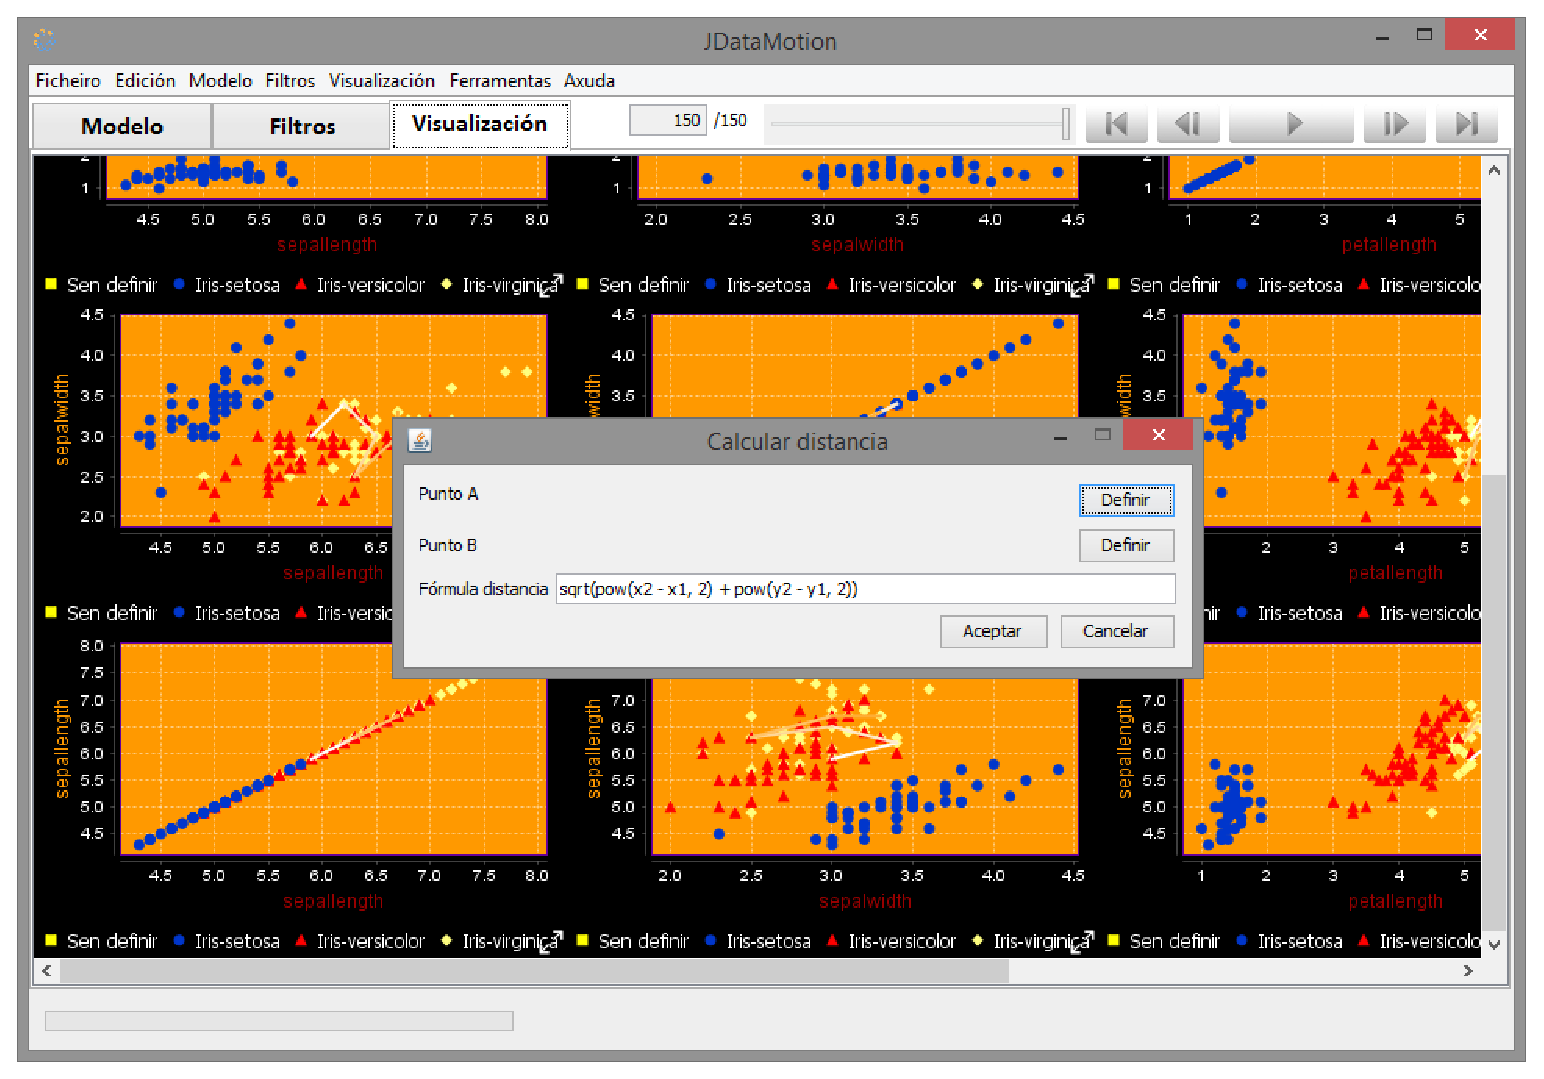
\includegraphics[width=\textwidth,height=\textheight,keepaspectratio]{figuras/calcularDistancia}
\caption{Menú calcular distancia}
\label{calcularDistancia}
\end{figure}

Para calcular a distancia entre dous puntos, temos que pinchar no botón ``Definir'' de cada un. Ao facelo, a aplicación prepararase para recibir as coordenadas de un punto pinchando enriba del no diagrama e premendo a continuación no cadro emerxente que detalla os seus atributos (pode haber varios puntos superpostos, e hai que especificar cal dos cadros emerxentes que o detalla é o que queremos seleccionar). Tamén teremos que definir a fórmula para achar a distancia. Para isto empregaremos \$1 para referenciar ao punto A e \$2 para refrenciar ao punto B. a continuación referenciaremos os seus atributos por medio de un punto e o atributo entre comiñas graves (\grave{}). Por exemplo: \$1.\grave{}sepallength\grave{}. A fórmula ten autocompletado, de forma que ao detectar a secuencia \$1. xa amosa unha lista cos atributos posibles do puntoA. Unha vez se definan os dous puntos e a fórmula da distancia, premendo Aceptar aparecerá un cadro de diálogo co resultado.

Para rematar, enriba do lenzo para os diagramas temos 5 botóns máis un desprazador. Utilizarémolos para controlar a reprodución dos datos.

O botón da esquina dereita, unha frecha cun tope, serve para colocarse no final da reprodución (todos os puntos representados).

O botón anterior, unha frecha cunha barra á sua esquerda, permítenos avanzar un paso na reprodución.

O botón central da inicio á reprodución. Si esta xa está producíndose, cambia a súa icona para pausala.

O segundo botón pola esquerda permítenos retroceder un paso na reprodución.

O último botón á esquerda serve para levar a reprodución ao seu principio (só un punto representado).

Podemos utlizar o desprazador que está en liña con estes botóns para acceder á fracción da reprodución que queiramos. Podemos manexalo arrastrando o pivote ou premendo nunha posición do desprazador para que o pivote vaia a ela.

\subsection{Outras funcionalidades}

Indo a Ficheiro \textgreater{} Pechar, poderemos pechar o programa. No menú ficheiro tamén temos outras posibilidades, que podemos activar no momento que desexemos durante a nosa experiencia. Por exemplo, podemos exportar o experimento actual cara un novo ficheiro en formato .csv ou .arff. Non está permitida a sobrescritura de ningún ficheiro, xa que ese ficheiro pode ter sesións gardadas que quedarían corruptas ao intentar restauralas.

Tamén podemos optar por gardar a sesión, almacenando todo o noso traballo para continuar máis tarde co programa no mesmo estado ca no momento no que se gardou a sesión.

O menú desfacer contén os ítems Desfacer e Refacer, cos que poderemos rectificar unha acción ou volver a realizala.

No menú de Ferramentas, o elemento Idioma permite definir o idioma da aplicación. Ao cambialo o programa reiniciarase, así que debemos previamente gardar a sesión ou exportar cara un ficheiro.

No menú Axuda temos unha entrada chamada Acerca de, que abre un diálogo con información sobre a aplicación e o seu desenvolvemento.